\documentclass{article}
\usepackage{graphicx}
\usepackage{tikz}
\usepackage{CJKutf8}
\usepackage{amsmath}
\usepackage{amsthm}
\renewcommand{\figurename}{图}
\begin{document}
\begin{CJK}{UTF8}{gbsn}
\newtheorem*{Ex}{习题}
\begin{Ex}
  一个图是可双色的当且仅当它没有奇数长的圈。
\end{Ex}
\begin{proof}[证明]
  设图$G$为可双色的,则显然图$G$没有奇数长的圈。这是因为假设图$G$有奇数长的圈$C$,
  则$C$是3色的,从而$\chi(G) \geq 3$,与$G$是可双色的矛盾。

  设图$G$没有奇数长的圈,以下给出一种用两种颜色对$G$的顶点进行着色的算法,从而证明图$G$是可双色的。不妨设图$G$是连通的,否则可以对图$G$的每个连通分量分别进行着色。任取$G$的一个顶点$a$,对其着红色,然后对与顶点$a$邻接的顶点着蓝色,接下来对所有与已经着色的顶点相邻接的顶点着红色,这样依次下去,每次都对所有与已经着色的顶点相邻接的顶点着与前一次的着色不同的另一种颜色。该算法结束时用至多两种颜色对$G$的顶点进行了着色,如图1所示。
  \begin{figure}
  \begin{minipage}{0.49\linewidth}
    \centering
  \includegraphics[width=4cm,height=3cm]{color25}    
    \caption{着色过程示意图}
    \label{fig:coloring}  
  \end{minipage}
  \begin{minipage}{0.49\linewidth}
  \centering
      \includegraphics[width=4cm,height=3cm]{color26}
  \caption{u和v的着色发生冲突的情况}
  \label{fig:collision}
  \end{minipage}
\end{figure}    
以下证明每次对所有与已经着色的顶点相邻接的顶点着与前一次的着色不同的另一种颜色时,
不会产生相邻的两个顶点着以相同颜色的情况,从而保证前面的算法是正确的。用反证法。
假设对顶点$u$进行着色时,不妨设对其着红色,已经有一个与之相邻的顶点$v$着了红色,
如图2所示。
从着色的过程知,从顶点$a$到顶点$u$之间有一条路$P_1$,其上的顶点依次着了红色和蓝色,
从顶点$a$到顶点$v$之间也有一条路$P_2$,其上的顶点依次着了红色和蓝色。
取$P_1$和$P_2$的最后一个公共的顶点$x$,则$P_1$上从顶点$u$到顶点$x$的路与$P_2$上从顶点$x$到顶点$v$的路和边$vu$一起构成一个圈,该圈上$u$和$v$着相同的颜色,其他各顶点依次着不同的颜色,因此其长度为奇数,与$G$中没有奇数长的圈矛盾。
  
\end{proof}
\end{CJK}
\end{document}

%%% Local Variables:
%%% mode: latex
%%% TeX-master: t
%%% End:
